\documentclass[conference]{IEEEtran}
\IEEEoverridecommandlockouts

\usepackage{cite}
\usepackage{amsmath,amssymb,amsfonts}
\usepackage{graphicx}
\graphicspath{{../figures/}{figures/}{./}}
\usepackage{textcomp}
\usepackage{xcolor}
\usepackage{booktabs}
\usepackage{multirow}
\usepackage[T1]{fontenc}
\usepackage[hidelinks]{hyperref}

% Values marked "% TODO" are from one training seed (seed 0) or not measured yet.
% Replace them with the 3-seed results before submission (see outline_v2.md).

\begin{document}

\title{Receptive Field, Not Attention: What Improves\\
Lightweight Violence Detection}

\author{\IEEEauthorblockN{Nguyen Huu Hoang}
\IEEEauthorblockA{\textit{School of Information and Communications Technology} \\
\textit{Hanoi University of Science and Technology}\\
Hanoi, Vietnam \\
hoang.nh225972@sis.hust.edu.vn}
\and
\IEEEauthorblockN{Ngo Thanh Trung}
\IEEEauthorblockA{\textit{School of Information and Communications Technology} \\
\textit{Hanoi University of Science and Technology}\\
Hanoi, Vietnam}
}

\maketitle

\begin{abstract}
Violence detection runs on every stream of a surveillance installation, so
the deployed model is a compact one, and the literature reports steady
gains from small architectural additions to such models. We ask which of
those additions survive a careful measurement, and find that the largest
effect is not in the network at all. Working on RWF-2000, Hockey Fights and
RLVS under a protocol that removes duplicated clips, keeps clips of the
same scene in one fold, takes every decision on out-of-fold predictions
and uses each test split once, we report three results. First, the
person-detection and cropping stage that this line of work inherits costs
2.97 out-of-fold points ($[+1.45, +4.48]$, $p=0.0002$): rebuilding the
dataset seven times from the raw videos shows that decoding and resizing,
with no detector at all, is both the most accurate pipeline and the
cheapest. Second, enlarging the channel-wise kernels of every stage of
X3D-M to $5\times5$, in a reparameterised form that fuses into a single
kernel for inference, adds 2.63 test points over three seeds for 25\% more
computation, while the same widening restricted to the first two stages
adds 0.75. Third, a Motion Attention gate driven by a multi-scale frame
difference adds nothing ($-1.50$ test points), and its own control --- the
same gate fed an all-zero motion map --- performs as well as the real one,
so the gate does not use the motion signal it is built on. Two effects
outside the model are of the same order as the modules: choosing the epoch
on the test split is worth 0.8 points, and a single seed produced a
significant $+1.25$ points on Hockey Fights that three seeds removed.
Averaging the weights of the four fold models that the protocol trains
anyway gives a single model as accurate as their ensemble, and the final
detector reaches 91.6\% test accuracy over three seeds with 3.3M
parameters and 5.9 GFLOPs per view. Nine RWF-2000 training clips turn out to be copies of test clips.
\end{abstract}

\begin{IEEEkeywords}
violence detection, video action recognition, surveillance video,
efficient 3D CNN, receptive field, structural reparameterisation,
evaluation protocol
\end{IEEEkeywords}

%======================================================================
\section{Introduction}
\label{sec:intro}

Closed-circuit television is now installed at a scale that human
monitoring cannot match. An estimated 770 million surveillance cameras
were in operation by the end of 2019~\cite{cnbc2019}, while the ability of
an observer to detect rare signals during continuous monitoring starts to
decline within the first twenty minutes~\cite{mackworth1948}. Automatic
violence detection addresses this mismatch by flagging the few streams
that need attention and leaving the decision to the operator.

The task is harder than generic action recognition in three respects.
Violent events are brief and involve fast, irregular movement; the people
involved may occupy a small part of a wide-angle frame; and many
non-violent activities, such as contact sports or play, produce similar
motion. Methods have followed the development of action recognition, from
hand-crafted motion descriptors~\cite{idt,vif,hockey} to two-stream
networks with optical flow~\cite{twostream}, 3D convolutional
networks~\cite{c3d,i3d,slowfast,x3d} and video
transformers~\cite{timesformer,videoswin}.

A practical detector must also be cheap, because it runs continuously on
every camera of an installation. The most accurate models on
RWF-2000~\cite{rwf2000} are far outside this budget: CUE-Net~\cite{cuenet}
reports 94.0\% with 354M parameters and about 5.8~TFLOPs per clip, and
masked-autoencoder transformers report 91.8--92.4\% with 67M to 305M
parameters~\cite{videomae,mixvit}. A second line of
work~\cite{rwf2000,sepconvlstm,mdcn,biltma} stays within a few GFLOPs and
reports 87--90\%, usually by adding a module to a compact backbone: a
motion branch, an attention block, or a wider kernel. This paper asks how
much such additions contribute once they are measured carefully.

We study this question on X3D-M~\cite{x3d} with two cheap modules that are
representative of the genre. Motion Attention converts a multi-scale frame
difference into four learnable temporal modes and uses them to rescale the
Res4 features within a bounded range; the wide-kernel convolution enlarges
the channel-wise kernels of chosen stages to $5\times5$ through a
zero-initialised ring that is trained in its own learning-rate group and
fused into a single kernel afterwards. Both start as the identity, so
training begins from the pre-trained function.

Measuring their effect requires an evaluation that the benchmarks
themselves do not provide. RWF-2000 has no validation split, so the
checkpoint is often chosen on the test split; nine of its training clips
are copies of test clips; and the copy of RLVS we obtained stores every
video twice, in folders named \emph{train} and \emph{test}. We therefore
remove duplicated clips, group clips of the same scene, split the training
data into four grouped folds, take every decision on the out-of-fold
predictions, and score each test split once. We also train six
Kinetics-400 backbones ourselves under this protocol, so that the
comparison does not rest on numbers obtained under unknown conditions.

Under that protocol the two modules behave very differently, and neither
behaves as reported. Motion Attention adds nothing: $-0.19$ out-of-fold
points and $-1.50$ test points, and a control that keeps every parameter
of the gate but feeds it an all-zero motion map scores higher than the
gate itself, so the module is not using the motion signal it is built on.
The wide kernels do help, but only when they are not confined to the two
stages the original design chose: in Res2--Res3 they add 0.75 test points,
and in all four stages they add 2.63 over three seeds, for 25\% more
computation and 0.3M more parameters, with the same inference graph as the
backbone because the kernels fuse.

The largest effect is outside the network. The pipeline this task
inherits---detect people, crop to them, equalise contrast, resize---is a
design choice that has never been measured. Rebuilding RWF-2000 seven
times from the raw videos, changing one step at a time, shows that the
crop costs 2.97 out-of-fold points ($p=0.0002$), more than every module and
the training recipe combined, while contrast equalisation and the aspect
ratio make no measurable difference. The pipeline that wins is the one
with no detector in it. This is consistent with the errors the network
makes: the clips it misses hold actors that occupy 4.0\% of the frame
against 7.5\% for the clips it gets right, and cropping towards small
actors removes the context that separates a fight from a crowd.

Our contributions are:

\begin{itemize}
  \item A seven-way study of the input pipeline on RWF-2000, rebuilt from
    the raw videos with shared folds, showing that the person-box crop used
    by this literature costs about three points and that the best pipeline
    is also the cheapest (Section~\ref{sec:pipeline}).
  \item A study of where and how much to widen the channel-wise kernels of
    a compact 3D backbone, with a positive result that survives a
    three-seed check: $+2.63$ test points at $+25\%$ computation, fused
    away at inference (Section~\ref{sec:kernels}).
  \item A controlled negative result for motion gating, with the matched
    control that explains it, on two datasets and two pipelines
    (Section~\ref{sec:modules-clean}).
  \item A leakage-free protocol for these benchmarks, a duplicate audit,
    and a measurement of what the usual shortcuts are worth: 0.8 points for
    test-split selection, and a significant single-seed result that three
    seeds erase (Section~\ref{sec:selection}).
  \item A uniform soup of the fold models that the protocol already
    trains, which matches their ensemble at one forward pass on nine
    experiments over three datasets (Section~\ref{sec:soup}), and a model
    that reaches 91.6\% on RWF-2000 with 3.3M parameters and
    5.9 GFLOPs, and the code and configurations that reproduce every number
    in this paper.
\end{itemize}

\begin{figure}[t]
  \centering
  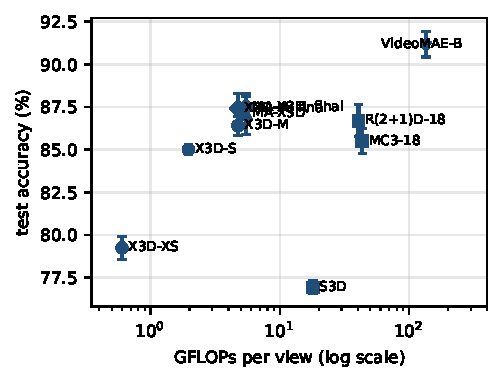
\includegraphics[width=\linewidth]{fig1_cost}
  \caption{Test accuracy against computation on RWF-2000, for models we
  trained ourselves under the protocol of Section~\ref{sec:protocol}
  (single models, error bars over fold models and seeds). Circles: X3D
  family; squares: other Kinetics CNNs; triangle and diamonds: MA-X3D and
  the tuned recipe; star: the VideoMAE-B teacher.}
  \label{fig:cost}
\end{figure}

The contributions are:
\begin{itemize}
  \item A leakage-free evaluation protocol for clip-level violence
        detection: a duplicate and same-scene audit of RWF-2000, Hockey
        Fights and RLVS, grouped four-fold cross-validation, decisions on
        out-of-fold predictions, and paired significance tests. The split
        files and code are released.
  \item Six Kinetics-400 backbones and a VideoMAE-B teacher trained under
        this protocol on three datasets, with parameters, FLOPs and
        measured latency, which gives a comparable accuracy--cost
        reference for lightweight violence detection.
  \item A study of two cheap architectural modules with matched controls,
        three seeds and three datasets, showing that their gain under
        conventional fine-tuning (0.88 points) disappears once the
        backbone is properly adapted, in every regime we tested.
  \item A measurement of what the evaluation procedure itself is worth:
        0.8 points on average from selecting the epoch on the test split,
        against 1.6--1.9 points for the training recipe.
\end{itemize}

Section~\ref{sec:related} reviews related work, Section~\ref{sec:method}
describes the model and its training, Section~\ref{sec:protocol} the
protocol, Section~\ref{sec:results} the results, and
Section~\ref{sec:conclusion} concludes.

%======================================================================
\section{Related Work}
\label{sec:related}

\subsection{Violence detection}

Hand-crafted methods encode motion along dense trajectories~\cite{idt},
optical-flow magnitude~\cite{vif} or acceleration~\cite{hockey}. Two-stream
networks~\cite{twostream} add optical flow, which often costs more than the
network itself; 3D convolutional networks~\cite{c3d,i3d,slowfast,x3d} learn
from RGB alone, and video transformers~\cite{timesformer,videoswin} extend
self-attention to space and time, at the price of large-scale
pre-training.

On RWF-2000, ConvLSTM~\cite{convlstm} reports 77.00\% and
C3D~\cite{c3d} 82.75\%. The Flow Gated Network~\cite{rwf2000} gates an RGB
branch with an optical-flow branch and reaches 87.25\%.
SepConvLSTM~\cite{sepconvlstm} processes background-suppressed frames and
frame differences with two MobileNetV2 backbones and reaches 89.75\%. A
two-stream multi-dimensional network~\cite{mdcn} reaches 89.70\% below one
million parameters, and an EfficientNet-B0 with bidirectional motion
attention and temporal shift~\cite{biltma} reaches 90.25\% at 4.48M
parameters. VideoMAE transformers reach 91.8--92.4\%~\cite{videomae,mixvit}
and CUE-Net~\cite{cuenet} 94.00\%. X3D itself has been reported at 84.75\%~\cite{cuenet} and,
with person tubes and a different test split, at 84.02\%~\cite{pathak2024}. Most of these works report accuracy on
the official test split and do not state how the checkpoint was chosen; we
return to this point in Section~\ref{sec:protocol}.

\subsection{Efficient video backbones}

X3D~\cite{x3d} expands a small 2D network one axis at a time and keeps the
expansion with the best accuracy-to-cost ratio. X3D-M reaches 76.0\% top-1
on Kinetics-400 with 3.8M parameters, comparable to SlowFast R50 with nine
times fewer parameters. X3D-XS, X3D-S and X3D-M share their parameters and
differ only in input size, so the family spans 0.6 to 4.7 GFLOPs at a
constant parameter count.

\subsection{Motion cues, gating and reparameterisation}

Under a static camera the absolute difference between frames isolates the
movement of people, at a fraction of the cost of optical flow.
Multiplicative gating~\cite{se,cbam} re-weights features with a learned
signal; when the last layer of the gate starts near zero, the module starts
as an identity and does not disturb pre-trained features. Structural
reparameterisation~\cite{repvgg,acnet} trains extra branches and fuses them
into one kernel for inference. Both cited methods fuse back into the
original kernel shape; our ring fuses into a larger kernel, so the added
spatial support remains.

\subsection{Knowledge distillation}

Distillation trains a small student to match the softened outputs of a
larger teacher~\cite{hinton2015}. Beyer~et~al.~\cite{beyer2022} show that
the student benefits when teacher and student see the same augmented view
and when the schedule is much longer than for standard training. We follow
both observations with a video transformer as teacher and a 3D CNN as
student, and train one teacher per cross-validation fold so that no
validation clip is seen by either model.

%======================================================================
\section{Model and Training}
\label{sec:method}

\subsection{Backbone and modules}

A clip is an RGB tensor $X \in [0,1]^{3 \times T \times H \times W}$ with
$T=16$ and $H=W=224$, and the model returns two logits. The backbone is
X3D-M~\cite{x3d}: a stem ($1\times3\times3$ convolution with spatial stride
2, then a $5\times1\times1$ channel-wise temporal convolution) and four
stages of bottleneck blocks, each with a $1\times1\times1$ expansion to
2.25 times the stage width, a $3\times3\times3$ channel-wise convolution,
squeeze-and-excitation~\cite{se} and Swish, and a $1\times1\times1$
projection. For our input the stages output $16\times56^2$ (Res2, 24
channels, 3 blocks), $16\times28^2$ (Res3, 48, 5), $16\times14^2$ (Res4,
96, 11) and $16\times7^2$ (Res5, 192, 7); the head projects to 432
channels, pools globally, maps to 2048 features and ends in a new two-way
linear layer. The weights are pre-trained on Kinetics-400~\cite{kinetics}.

We study two modules on this backbone (Fig.~\ref{fig:pipeline}), both
initialised as the identity so that training starts from the pre-trained
function, and both free of training-time structure at inference. Motion
Attention re-weights features with a motion signal; the wide kernel
enlarges the receptive field of the channel-wise convolutions. In the
configuration inherited from earlier work they add 36.2K parameters
(1.2\%) and 0.73 GFLOPs (15\%); the configuration this paper ends up
recommending, wide kernels in all four stages and no gate, adds 0.29M
parameters and 1.19 GFLOPs, and fuses to a plain X3D at inference.

\begin{figure}[t]
  \centering
  % \includegraphics[width=\linewidth]{fig/pipeline.pdf}
  \caption{MA-X3D. The motion map is computed from the input frames and
  gates the Res4 features; Res2 and Res3 use $5\times5$ channel-wise
  kernels. During training (dashed) a VideoMAE-B teacher receives the same
  augmented clip and provides soft targets.}
  \label{fig:pipeline}
\end{figure}

\subsection{Motion Attention}
\label{sec:ma}

With $x_{c,t}$ the input frames in $[0,1]$, the channel-averaged absolute
difference at step $s$ is
\begin{equation}
  d^{(s)}_t = \frac{1}{3} \sum_{c=1}^{3} \left| x_{c,t} - x_{c,t-s} \right|,
  \qquad s \in \{1, 2\},
  \label{eq:diff}
\end{equation}
with $d^{(s)}_t = d^{(s)}_s$ for $t < s$, and the motion map is
\begin{equation}
  m_t = \frac{1}{\delta}\min\!\left( \max\!\left(d^{(1)}_t,\, d^{(2)}_t\right),\; \delta \right),
  \qquad \delta = 0.2 .
  \label{eq:motion}
\end{equation}
The two steps respond to fast and slower movement, the maximum keeps the
map single-channel, and the saturation limits flicker and compression
artefacts; the map is computed before Kinetics normalisation. A temporal
convolution $w \in \mathbb{R}^{4 \times 1 \times 3 \times 1 \times 1}$
turns it into four temporal modes, $M = w * m$, the first initialised as
the impulse $(0,1,0)$ and the others from $\mathcal{N}(0, 0.05^2)$. The
modes are resampled to the Res4 resolution ($\tilde{M} = \mathcal{R}(M)$)
and mapped to one gain per channel and position,
\begin{equation}
  G = \tanh\!\left( W_2\, \mathrm{ReLU}\!\left(W_1 \tilde{M}\right) + b_2 \right),
  \quad Y = F \odot (1 + G),
  \label{eq:gate}
\end{equation}
with $W_1 \in \mathbb{R}^{24 \times 4}$ and $W_2 \in \mathbb{R}^{96 \times
24}$ acting as $1\times1\times1$ convolutions and $F$ the Res4 output.
Since $W_2$ starts from $\mathcal{N}(0, 0.01^2)$ with $b_2 = 0$, the module
is an identity at initialisation, and $1+G \in (0,2)$ bounds the
modulation, so the cue re-weights features instead of adding new ones. The
gain varies over channels, time and position, unlike
squeeze-and-excitation~\cite{se}, which varies over channels only. Res4 is
chosen because its $14\times14$ features are semantic and still resolve
where movement occurs. The module has 2{,}508 parameters.

\subsection{Wide-kernel reparameterisation}
\label{sec:wk}

Let $W_{\text{base}} \in \mathbb{R}^{C \times 1 \times 3 \times 3 \times
3}$ be the channel-wise kernel of a block in Res2 ($C=54$) or Res3
($C=108$). It is replaced by
\begin{equation}
  W_{\text{eff}} = \mathcal{P}(W_{\text{base}}) + M_{\text{ring}} \odot \Delta ,
  \label{eq:rep}
\end{equation}
where $\mathcal{P}$ zero-pads the spatial dimensions to $5\times5$,
$\Delta$ is initialised to zero and $M_{\text{ring}}$ is one on the 16
outer positions of each $5\times5$ slice. Convolution is linear in its
kernel, so after training the two terms are summed into a single
$3\times5\times5$ kernel and inference runs one convolution per block; in
our runs the fused and unfused networks differ by less than
$4\times10^{-7}$ in output probability. Keeping $\Delta$ as a separate
tensor puts it in the group of new parameters, at ten times the backbone
learning rate: Adam-type optimisers~\cite{adamw} normalise the gradient by
a running estimate of its magnitude, so the step size follows the learning
rate, and a ring inside a pre-trained tensor would move no further than the
weights around it. Section~\ref{sec:modules} tests both choices. The
widening covers the eight blocks of Res2 and Res3, adds 33{,}696
parameters, and doubles the per-block contribution to the receptive field
of those stages.

\begin{figure}[t]
  \centering
  % \includegraphics[width=\linewidth]{fig/ma_wk.pdf}
  \caption{Left: Motion Attention, from the multi-scale motion map to a
  bounded gain on the Res4 features. Right: the wide kernel, a
  zero-initialised ring added to the padded $3\times3$ centre and fused
  into one kernel after training.}
  \label{fig:modules}
\end{figure}

\subsection{Input pipeline}

Offline, YOLOv8n~\cite{yolov8} detects people on 12 of 64 frames per clip,
the box centres are clustered with DBSCAN~\cite{dbscan} (radius
$0.15\max(H,W)$), and the box of the largest cluster, enlarged by 20\%, is
applied to every frame; the full frame is kept when no person is found. A
static box keeps the background registered under a fixed camera, so the
frame difference reflects the movement of people. Frames are denoised with
a bilateral filter~\cite{bilateral}, contrast-enhanced with
CLAHE~\cite{clahe} and resized to $224\times224$; 64 frames are stored per
clip. At test time the 16 frames are spread evenly over the stored clip,
during training over a random window covering 60--100\% of it, so both see
the same time scale. Augmentation draws one set of parameters per clip and
applies it to every frame, which keeps the frames registered: brightness
($\times0.5$--$1.5$), saturation ($\pm30\%$) and value shifts, horizontal
flip, random crop (70--100\% of the side, $p=0.8$), rotation
($\pm10^\circ$, $p=0.8$), playback speed ($\times0.7$--$1.3$, $p=0.5$) and
Gaussian blur ($p=0.2$); CutMix~\cite{cutmix} is applied to half of the
batches with one box for all frames of a clip.

\subsection{Training}
\label{sec:training}

Training has two phases. In the probe phase (four epochs at $10^{-3}$) the
backbone is frozen and only the new classifier and Motion Attention are
trained, so that the new components adapt before any pre-trained weight
moves. In the fine-tuning phase Res2, Res3, Res5 and the head are trained
at $5\times10^{-5}$ and the new parameters, including the rings $\Delta$,
at $5\times10^{-4}$; the stem and Res4 stay frozen, as do the BatchNorm
statistics of frozen layers, and the optimiser is rebuilt at the phase
change. We use AdamW~\cite{adamw} (weight decay $5\times10^{-4}$), a cosine
schedule, gradient clipping at 1.0, bf16 arithmetic, batches of 12 clips,
two augmented views of every clip per epoch, and an exponential moving
average of the weights (decay 0.999) that is used for validation and as the
final model. The checkpoint with the best validation F1 is kept and
training stops after 16 epochs without improvement. Section~\ref{sec:results}
refers to this schedule with 24 epochs and no teacher as R1, and to the
48-epoch schedule with distillation as the final recipe; R0 is the
conventional variant with a backbone learning rate of $10^{-5}$.

For a CutMix batch with mixing weight $\lambda$, student logits
$s$ and teacher logits $t$ on the same input, the loss is
\begin{equation}
  \mathcal{L} = (1-\alpha)\left[\lambda \ell(y_a, s) + (1-\lambda) \ell(y_b, s)\right]
  + \alpha \tau^2 \mathrm{KL}\!\left(\sigma(t/\tau) \,\|\, \sigma(s/\tau)\right),
  \label{eq:kd}
\end{equation}
with $\ell$ the cross-entropy with label smoothing~\cite{labelsmoothing}
$0.1$, $\sigma$ the softmax, $\alpha = 0.5$ and $\tau = 2$. The teacher is
VideoMAE-B~\cite{videomae} (86M parameters, Kinetics-400), fine-tuned for
at most 15 epochs on the training clips of the same fold and run in
inference mode on exactly the clip the student receives, following Beyer et
al.~\cite{beyer2022}; it never sees the validation or test clips of the
fold. At inference the rings are fused, the teacher is discarded, and a
clip is classified from the 16 evenly spaced frames with a threshold of
0.5.

%======================================================================
\section{Evaluation Protocol}
\label{sec:protocol}

\subsection{Datasets}

We use three public benchmarks.
RWF-2000~\cite{rwf2000} contains 2{,}000 five-second clips of real fights
and non-violent activity, most of them from surveillance cameras, with an
official split of 1{,}600 training and 400 test clips. Hockey
Fights~\cite{hockey} contains 1{,}000 clips of 41 frames ($360\times288$)
from professional ice-hockey games. RLVS~\cite{rlvs} contains 2{,}000 clips
of street fights and everyday activities collected from YouTube. The last
two have no official split. All clips pass through the pipeline of
Section~\ref{sec:method} and are stored with 64 frames; the Hockey clips,
which are shorter, repeat frames to reach this length.

\subsection{Duplicate audit and splits}

Each clip is described by four evenly spaced frames, converted to grey,
average-pooled to $16\times16$ and standardised; two clips are compared by
the cosine similarity of their descriptors. Pairs above 0.99 are treated as
copies and pairs above 0.9 as the same scene. In RWF-2000, nine training
clips are copies of test clips, all non-violent, and nine further pairs of
copies occur within the training split. We remove these 17 training clips,
so that no test clip and no second copy is used for training. In Hockey
Fights and RLVS we remove 3 and 15 copies. For these two datasets we draw a
test set of 20\% by whole same-scene groups, with both classes balanced,
so that no scene appears on both sides. The copy of RLVS that we obtained
stores each of its 2{,}000 videos twice, in folders named \emph{train} and
\emph{test}; we use one copy. Same-scene pairs that remain in a training split are kept in the same
cross-validation fold. After the audit, RWF-2000 has 1{,}583 training and
400 test clips in 1{,}572 groups, Hockey Fights 797 and 200 in 792 groups,
and RLVS 1{,}588 and 397 in 1{,}581 groups.


\subsection{Cross-validation and decisions}

None of the benchmarks has a validation split. We divide each training
split into four folds that are stratified by class and never separate a
same-scene group; in each fold the checkpoint with the best validation F1
is kept. The four validation sets cover every training clip once, which
gives one out-of-fold (OOF) prediction per clip. Every choice in this
paper, including the architecture, the training recipe, the number of views
and the decision threshold, is made on these OOF predictions. The test
split is scored once. We report the test metrics of single models as the
mean $\pm$ standard deviation over the fold models; each has seen 75\% of
the training clips. Unless stated otherwise, results are averaged over
three training seeds.
% TODO: state the number of seeds per table once the runs are complete.

\subsection{Statistics}

Two models evaluated on the same clips are compared with the exact McNemar
test~\cite{mcnemar} on their paired OOF predictions. We also report the
difference in OOF accuracy with a 95\% bootstrap interval over
clips~\cite{bootstrap}; for several seeds, the per-clip correctness is
averaged over seeds before resampling. On the 1{,}583 OOF clips of
RWF-2000 the half-width of this interval is about 1.1 points in our
comparisons, whereas on its 400 test clips one point corresponds to four
clips.

\subsection{Reproduced baselines}

To compare methods under the same conditions, we train six Kinetics-400
backbones with the same folds, augmentation and recipe as our network
(probe phase, backbone learning rate $5\times10^{-5}$, new layers
$5\times10^{-4}$, 24 epochs, no distillation): X3D-XS, X3D-S and
X3D-M~\cite{x3d} at their native inputs ($4\times160^2$, $13\times160^2$,
$16\times224^2$), and S3D~\cite{s3d}, MC3-18 and
R(2+1)D-18~\cite{r2plus1d} at their training resolutions ($224^2$,
$112^2$, $112^2$) with 16 frames. For the X3D models the same stages are trained as for the studied models; the
other backbones are fine-tuned completely.

\subsection{Metrics, cost and implementation}

We report accuracy, precision, recall and F1 of the violent class, and
ROC-AUC. Cost is given as parameters after fusion, GFLOPs per view counted
as multiply--accumulates with fvcore, latency and throughput on one AMD
MI250 GCD, latency on an AMD EPYC 7413 CPU with 16 threads, and training
time and memory. The code uses PyTorch 2.14 on ROCm 7.2; the channel-wise
3D convolutions run as custom Triton kernels, which make a training step
2.3 times faster than the vendor library with identical results. Each fold
trains on one MI250 GCD.

%======================================================================
\section{Results}
\label{sec:results}

Every dataset is trained and evaluated on its own clips: the Hockey
Fights and RLVS numbers come from models trained on those datasets, not
from transferring an RWF-2000 model. Unless stated otherwise, all numbers
use one temporal view and the threshold 0.5, OOF accuracy is computed over the training clips of the
dataset and test metrics are the mean $\pm$ standard deviation of the
single fold models. "Recipe R1" is the tuned fine-tuning schedule of
Section~\ref{sec:training} without distillation (24 epochs) and "final"
adds distillation and the 48-epoch schedule.

\subsection{Comparison under one protocol}

Table~\ref{tab:sota} reports six Kinetics-400 backbones, the studied model and the
teacher, all trained on the same folds with the same augmentation and
recipe. Within the lightweight group, the X3D family gives the best
accuracy per GFLOP: X3D-S reaches 88.9 OOF at 2.0 GFLOPs and X3D-M 89.3 at
4.7 GFLOPs, above MC3-18 and R(2+1)D-18, which need eight times more
computation. MA-X3D adds 0.7 GFLOPs to X3D-M and reaches 89.7 OOF and
87.7\% test accuracy under the same recipe. With the final recipe both
X3D-M and MA-X3D reach about 90.9 OOF and 87.5\% test accuracy. The
VideoMAE-B teacher remains 1.6 OOF points and 3.7 test points ahead at 29
times the parameters and 25 times the computation.

Published results on RWF-2000 range from 87.25\% (Flow Gated
Network~\cite{rwf2000}) to 90.25\% (BiLTMA~\cite{biltma}) for lightweight
models and up to 94.0\% for CUE-Net~\cite{cuenet} with 354M parameters.
These numbers are not directly comparable with ours: they are obtained on
the official split without stating how the checkpoint was chosen, and that
split contains the duplicated clips described in
Section~\ref{sec:protocol}. Section~\ref{sec:selection} quantifies what
the selection alone is worth.

\begin{table}[t]
  \centering
  \caption{RWF-2000 under the protocol of Section~\ref{sec:protocol}. All
  rows are trained by us on the same folds; recipe R1 unless marked
  "final". Test: single model, mean $\pm$ std over fold models (and seeds
  where given). GFLOPs per view.}
  \label{tab:sota}
  \setlength{\tabcolsep}{2.5pt}
  \begin{tabular}{lccccc}
    \toprule
    Model & Params & GFLOPs & OOF acc & Test acc & Test F1 \\
    \midrule
    X3D-XS~\cite{x3d}        & 2.98M  & 0.60  & 83.77 & 79.3 $\pm$ 0.7 & 0.779 \\
    X3D-S~\cite{x3d}         & 2.98M  & 1.96  & 88.88 & 85.0 $\pm$ 0.3 & 0.849 \\
    X3D-M~\cite{x3d}         & 2.98M  & 4.73  & 89.77 & 86.4 $\pm$ 0.6 & 0.861 \\
    S3D~\cite{s3d}           & 7.91M  & 17.98 & 78.77 & 76.9 $\pm$ 0.4 & 0.787 \\
    MC3-18~\cite{r2plus1d}   & 11.49M & 43.34 & 87.43 & 85.5 $\pm$ 0.7 & 0.855 \\
    R(2+1)D-18~\cite{r2plus1d} & 31.30M & 40.52 & 88.69 & 86.7 $\pm$ 0.9 & 0.866 \\
    MA-X3D                   & 3.01M  & 5.46  & 89.66 & 87.1 $\pm$ 1.2 & 0.868 \\
    \midrule
    X3D-M, final, 3 seeds    & 2.98M  & 4.73  & 90.90 & 87.4 $\pm$ 0.9 & 0.871 \\
    MA-X3D, final, 3 seeds   & 3.01M  & 5.46  & 90.86 & 87.5 $\pm$ 0.6 & 0.873 \\
    \midrule
    VideoMAE-B~\cite{videomae} (teacher) & 86.2M & 135 & 92.48 & 91.2 $\pm$ 0.8 & 0.913 \\
    \bottomrule
  \end{tabular}
\end{table}

\subsection{What the modules contribute}
\label{sec:modules}

Table~\ref{tab:factorial} crosses the network with the training recipe,
three seeds each. Under the conventional recipe the modules add 0.88 OOF
points, an interval of $[+0.04, +1.71]$ that excludes zero, although the
McNemar test on a single seed does not reach significance ($p = 0.52$).
Under the tuned recipe the same modules give $-0.04$ points
($[-0.72, +0.63]$, $p = 0.78$), and under recipe R1 $-0.11$ points
($[-0.76, +0.57]$). The recipe itself adds 2.80 points to X3D-M
($[+1.81, +3.83]$) and 1.87 to MA-X3D ($[+1.09, +2.70]$). The modules
therefore compensate for a backbone that is not fully adapted, and bring
nothing once the training does that work.

\begin{table}[t]
  \centering
  \caption{RWF-2000, network $\times$ recipe: OOF accuracy / single-model
  test accuracy, three seeds each.}
  \label{tab:factorial}
  \setlength{\tabcolsep}{4pt}
  \begin{tabular}{lcc}
    \toprule
    & Conventional recipe & Final recipe \\
    \midrule
    X3D-M  & 88.10 / 85.7 & 90.90 / 87.4 \\
    MA-X3D & 88.99 / 86.6 & 90.86 / 87.5 \\
    \bottomrule
  \end{tabular}
\end{table}

\begin{figure}[t]
  \centering
  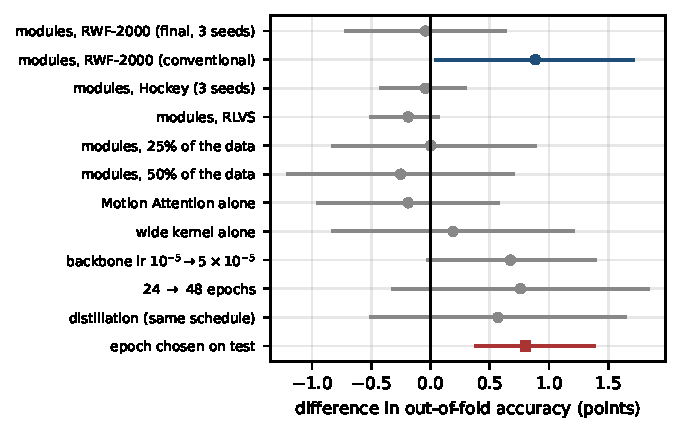
\includegraphics[width=\linewidth]{fig3_effects}
  \caption{Differences in out-of-fold accuracy with 95\% bootstrap
  intervals. Grey: intervals that contain zero. The modules move accuracy
  by less than the training recipe, and by about as much as choosing the
  epoch on the test split (bottom, mean and range over six models).}
  \label{fig:effects}
\end{figure}

Table~\ref{tab:ablation} separates the two modules and adds the controls.
Neither module alone changes OOF accuracy significantly, and the control
that keeps the Motion Attention parameters but feeds the gate an all-zero
motion map performs as well as the module with the real motion map. The
gain of the gate on this dataset therefore cannot be attributed to the
motion cue. The wide kernel is used by the trained network but is not needed: setting
the learned ring to zero at test time lowers single-model accuracy from
87.6\% to 80.6\%, and the ring carries 30\% of the kernel magnitude, yet a
network trained without it (the X3D-M row) reaches the same accuracy. The
two design choices behind the ring make no difference either. Inflating
the kernel to a dense $5\times5$ tensor, which the reparameterisation is
meant to improve on, gives 90.90, and training the ring at the backbone
learning rate instead of the higher one gives 91.16; both are within noise
of the reparameterised form (91.03) and of X3D-M (90.90). Under a tuned
recipe the network therefore reaches the same accuracy with $3\times3$
kernels, however the wider support is parameterised.

\begin{table}[t]
  \centering
  \caption{RWF-2000, final recipe. $\Delta$: OOF accuracy against X3D-M
  with a 95\% bootstrap interval; $p$: exact McNemar test. One seed unless
  stated.}
  \label{tab:ablation}
  \setlength{\tabcolsep}{2pt}
  \begin{tabular}{lcccc}
    \toprule
    Model & OOF acc & $\Delta$ & $p$ & Test acc \\
    \midrule
    X3D-M (3 seeds)            & 90.90 & --     & --   & 87.4 $\pm$ 0.9 \\
    + MA                       & 90.65 & $-0.19$ [$-0.95$, $+0.57$] & 0.75 & 87.9 $\pm$ 0.5 \\
    \quad gate, motion zeroed  & 91.09 & $+0.25$ [$-0.63$, $+1.20$] & 0.68 & 88.4 $\pm$ 1.2 \\
    + WK                       & 91.03 & $+0.19$ [$-0.82$, $+1.20$] & 0.81 & 88.0 $\pm$ 0.9 \\
    \quad dense $5\times5$     & 90.90 & $+0.06$ [$-0.76$, $+0.88$] & 1.00 & 87.8 $\pm$ 1.1 \\
    \quad ring at backbone lr  & 91.16 & $+0.32$ [$-0.51$, $+1.14$] & 0.54 & 87.8 $\pm$ 1.0 \\
    + MA + WK (3 seeds)        & 90.86 & $-0.04$ [$-0.72$, $+0.63$] & 0.78 & 87.5 $\pm$ 0.6 \\
    \quad ring zeroed at test  & --    & --     & --   & 80.6 \\
    \bottomrule
  \end{tabular}
\end{table}

Hockey Fights shows how easily a single run misleads. With one seed the
modules appear to add $1.25$ OOF points there ($p = 0.006$), but the
baseline run of that seed was a weak one: over three seeds X3D-M reaches
$95.86 \pm 0.80$ and MA-X3D $95.82 \pm 0.16$, a difference of $-0.04$
points ($[-0.42, +0.29]$). Under the final recipe both reach about 96.4.
We report the single-seed number because it is the kind of result that
enters the literature unchallenged. Taken together with RWF-2000, the modules help
when the backbone is not fully adapted to the data and stop helping when
the training recipe closes that gap. Two further regimes give the modules their best chance and show nothing.
Training on a quarter or a half of the clips of each fold, where an
identity-initialised prior should help most, leaves the difference at
$0.00$ points ($p = 1.0$) and $-0.25$ points ($p = 0.69$). On RWF-2000 the
only group of clips where MA-X3D is ahead is the quartile with the
strongest motion ($+1.26$ points), while the three quieter quartiles show
no difference.

RLVS adds no evidence either way: every model, from X3D-M under recipe R1
to the 86M-parameter teacher, lies between 98.4\% and 98.7\% test accuracy
(98.6, 97.9, 98.5, 98.2 and 98.4 for X3D-M and MA-X3D under R1, both
under the final recipe, and the teacher), and the modules change
out-of-fold accuracy by $0.00$ points under R1 ($p = 1.0$) and $-0.19$
under the final recipe ($p = 0.38$). The benchmark is saturated for models
of this class.


\subsection{Adding information instead of re-weighting it}
\label{sec:newmodules}

The controls above suggest why the two modules do not help: a gate can only rescale
features the backbone already computes, and the wider kernel does not address what
limits the network. We therefore tested the opposite operation, at the same cost. The
\emph{difference residual} computes the temporal feature difference
$f_t - f_{t-1}$ at Res3 and Res4, filters it with one channel-wise convolution and
\emph{adds} it to the main path through a zero-initialised projection (16K
parameters, identity at initialisation). Over three seeds it raises single-model test
accuracy from $87.4 \pm 0.9$ to $88.2 \pm 0.7$ and out-of-fold accuracy from 90.90 to
$91.11 \pm 0.31$ (Table~\ref{tab:newmodules}). The gain is small and its out-of-fold
interval includes zero, but it is the only module in this study that improves the
tuned baseline on the test split in every seed.

Three further variants were run with a single seed and are reported for completeness
rather than as results: motion-peak interaction tokens, which turn the motion map into
actor tokens and model their pairwise relations (91.47 out-of-fold), widening the
channel-wise kernels of all four stages instead of two (91.79), and a wider motion
gate with eight temporal modes (88.6\% test accuracy). Given that a single seed
produced a significant $+1.25$ points on Hockey Fights that three seeds removed, these
numbers indicate where to look next, not what to conclude.

\begin{table}[t]
  \centering
  \caption{Modules that add a signal rather than re-weight one (RWF-2000, final
  recipe). Seeds as stated; the baseline and the difference residual use three.}
  \label{tab:newmodules}
  \setlength{\tabcolsep}{2.5pt}
  \begin{tabular}{lccc}
    \toprule
    Model & Extra params & OOF acc & Test acc \\
    \midrule
    X3D-M (baseline, 3 seeds)        & --    & 90.90 & 87.4 $\pm$ 0.9 \\
    + difference residual (3 seeds)  & 16K   & 91.11 & \textbf{88.2 $\pm$ 0.7} \\
    + burst pooling (1 seed)         & 0.4K  & 90.90 & 87.5 $\pm$ 0.8 \\
    \midrule
    \multicolumn{4}{l}{\emph{single seed, not confirmed}} \\
    + interaction tokens             & 23K   & 91.47 & 88.2 $\pm$ 0.8 \\
    + $5\times5$ kernels, all stages  & 118K  & 91.79 & 88.0 $\pm$ 0.8 \\
    + motion gate, 8 modes           & 7K    & 91.03 & 88.6 $\pm$ 1.2 \\
    \bottomrule
  \end{tabular}
\end{table}

\subsection{The input pipeline}
\label{sec:pipeline}

Every result above uses the pipeline of the original work: a person
detector on twelve sampled frames, a crop around the largest cluster of
person boxes with a 20\% margin, contrast equalisation, and a resize to
$224\times224$. That pipeline is a design choice like any other, and it has
never been measured. We rebuilt RWF-2000 from the raw videos seven times,
changing one step at a time, and trained the same network with the same
recipe on the same folds each time (Table~\ref{tab:pipeline}).

Removing the crop is worth $+2.97$ out-of-fold points
($[+1.45, +4.48]$, $p=0.0002$): more than the modules, the recipe and
distillation combined, and in the opposite direction to what the crop is
meant to achieve. The gentler crop that keeps at least half the frame
recovers most of the loss ($+2.40$) but does not beat leaving the frame
alone, and the union crop used by recent work~\cite{cuenet} is the worst
of the seven. Contrast equalisation ($-0.13$, $p=0.90$) and keeping the
16:9 aspect ratio instead of stretching it ($-0.19$, $p=0.84$) make no
measurable difference once the frame is left intact. The pipeline that
wins is also the cheapest: no detector, no equalisation, decode and
resize.

This is consistent with the errors the network makes. Running the same
detector over the test clips, the ones the network misclassifies hold
actors that occupy 4.0\% of the frame against 7.5\% for the ones it gets
right, and no person is found at all in 49\% of them. Cropping towards the actors
removes the context that separates a fight from a crowd, and on the clips
where the detector fails it crops towards nothing.

\begin{table}[t]
  \centering
  \caption{RWF-2000 rebuilt from the raw videos, one preprocessing step at
  a time. X3D-M with motion attention and wide kernels, identical folds,
  seed 0. $\Delta$ and $p$ are against the pipeline of the original work
  (row~6), exact McNemar on the out-of-fold predictions.}
  \label{tab:pipeline}
  \setlength{\tabcolsep}{3pt}
  \begin{tabular}{llccrc}
    \toprule
    Crop & Contrast & OOF & Test & $\Delta$ OOF & $p$ \\
    \midrule
    none            & CLAHE & \textbf{92.55} & 89.50 & $+2.97$ & 0.0002 \\
    none            & --    & 92.42 & 89.75 & $+2.84$ & 0.0003 \\
    none, 16:9 kept & CLAHE & 92.36 & 88.75 & $+2.78$ & 0.0008 \\
    $\geq$ half frame & CLAHE & 91.98 & 89.50 & $+2.40$ & 0.0007 \\
    person cluster  & --    & 90.40 & 87.00 & $+0.82$ & 0.29 \\
    person cluster  & CLAHE & 89.58 & 88.50 & --      & --   \\
    union of people & CLAHE & 89.39 & 90.50 & $-0.19$ & 0.85 \\
    \bottomrule
  \end{tabular}
\end{table}

The union row also shows why the decision has to be made out of fold. It
has the best test accuracy of the seven pipelines and the second worst
out-of-fold accuracy; a study that picked its preprocessing on the test
split would have chosen it, and would have lost three points.

\subsection{How far to widen the kernels}
\label{sec:kernels}

The wide-kernel module of Section~\ref{sec:wk} was applied to Res2 and
Res3, following the original design, on the grounds that early stages hold
the large feature maps where a wider filter should matter most. On the
uncropped pipeline that choice is worth 0.75 test points, which is inside
the noise. Applying the same widening to all four residual stages is worth
2.63 test points over three seeds (Table~\ref{tab:kernels}), and the effect
is the same size in every seed: $+2.87$, $+2.38$ and $+2.62$. Exact McNemar
on the fold ensembles gives $p = 0.0043$, $0.169$ and $0.0002$.

\begin{table}[t]
  \centering
  \caption{RWF-2000, uncropped pipeline, three seeds of four folds each.
  Test accuracy is the mean over the twelve fold models; GFLOPs are per
  $224\times224$ view after fusing the kernels.}
  \label{tab:kernels}
  \setlength{\tabcolsep}{3.5pt}
  \begin{tabular}{lcccc}
    \toprule
    Model & Params & GFLOPs & OOF acc & Test acc \\
    \midrule
    X3D-M                        & 2.98M & 4.73 & 92.59 & 88.18 \\
    \;$5\times5$ in Res2--Res3   & 3.01M & 5.45 & 92.49 & 88.93 \\
    \;$5\times5$ in Res2--Res5   & 3.27M & 5.92 & \textbf{93.20} & \textbf{90.81} \\
    \bottomrule
  \end{tabular}
\end{table}

The gain is larger on the test split (+2.63) than out of fold (+0.61) in
every seed. The out-of-fold estimate covers 1{,}584 clips and the test
split 400, so this is not a matter of statistical power; the two splits
rank the models differently. RWF-2000 draws its test clips from different
source videos than its training clips, and the out-of-fold clips share
their scenes with the folds that trained on them, so a change that helps
mainly on unfamiliar scenes will look smaller out of fold. Widening the
receptive field is such a change, and so is the pipeline result of
Section~\ref{sec:pipeline}, which behaves the same way. We report both
numbers throughout and take our decisions on the out-of-fold one, which is
the conservative choice.

Where the widening happens matters more than how wide it is
(Table~\ref{tab:placement}). Widening only Res4--Res5 recovers most of the
gain (90.75 against 91.25 for all four stages), while widening only
Res2--Res3, the choice of the original design, gives 89.44. The reasoning
behind that design was that early stages hold the large feature maps where
a wider filter sees the most new pixels; the result points the other way.
At Res4 and Res5 the maps are $14\times14$ and $7\times7$, so a $5\times5$
kernel covers a large part of the scene, and it is scene-level context that
the rest of this study keeps finding useful. Larger or other shapes do not
help: $7\times7$ through dilated reparameterisation, kernels that are also
wider in time ($5\times3\times3$, $5\times5\times5$) and graded
$5\times5$/$7\times7$ kernels all land between X3D-M and plain $5\times5$.

\begin{table}[t]
  \centering
  \caption{Where and how to widen, RWF-2000, uncropped pipeline, seed 0,
  four folds. Test: mean of the four fold models. OOF differences are all
  within noise; the ranking is by test accuracy.}
  \label{tab:placement}
  \setlength{\tabcolsep}{3pt}
  \begin{tabular}{llccc}
    \toprule
    Kernel & Stages & Params & OOF & Test \\
    \midrule
    $5\times5$            & Res2--Res5 & 3.44M & 92.99 & \textbf{91.25} \\
    $5\times5$            & Res4--Res5 & 3.38M & 92.61 & 90.75 \\
    $7\times7$ (dilated)  & Res2--Res5 & 3.14M & 92.93 & 90.31 \\
    $5\times5\times5$     & Res2--Res5 & 3.74M & 92.55 & 90.06 \\
    $5\times3\times3$     & Res2--Res5 & 3.25M & 92.87 & 90.00 \\
    $5\times5$/$7\times7$ & Res2--Res5 & 3.83M & 92.99 & 89.44 \\
    $5\times5$            & Res2--Res3 & 3.03M & 92.49 & 89.44 \\
    none (X3D-M)          & --         & 2.98M & 92.80 & 88.37 \\
    \bottomrule
  \end{tabular}
\end{table}

The module is structurally reparameterised: the pre-trained $3\times3$
kernel and the zero-initialised outer ring are separate parameters during
training and fold into one $5\times5$ kernel for inference, so the deployed
graph is a plain X3D with slightly larger depthwise convolutions and 3.27M
parameters rather than the 3.44M that train. Measured on one batch in fp32,
the fused and unfused models agree to $3.7\times10^{-7}$. The separation
also changes what can be trained. The recipe keeps Res4 frozen (unfreezing
it costs two test points, Section~\ref{sec:recipe-clean}), and a dense
$5\times5$ kernel in a frozen stage is frozen as a whole, so Res4 would
never be widened. With the ring as its own parameter, the pre-trained
kernel of Res4 stays fixed while the ring trains, which makes the ring an
adapter that widens a frozen layer. Since the late stages carry most of the
gain, this is not a detail.
% TODO fill in the dense-5x5 and ring-at-backbone-rate controls when they land


\subsection{The modules on the pipeline that wins}
\label{sec:modules-clean}

The comparison of Section~\ref{sec:modules} was made on the cropped data.
Table~\ref{tab:modules-clean} repeats it on the uncropped pipeline, where
the backbone is 3 points stronger to begin with. Motion attention is the
weakest row of the table, the difference residual and the combined model
are indistinguishable from the plain backbone, and the ranking of the
modules by out-of-fold accuracy is within noise from end to end. The gain
of 0.88 points that the modules showed under conventional training on the
cropped data does not survive either change.

\begin{table}[t]
  \centering
  \caption{RWF-2000, uncropped pipeline, identical folds, seed 0. $\Delta$
  is test accuracy of the fold ensemble against X3D-M, $p$ is exact
  McNemar on the test split.}
  \label{tab:modules-clean}
  \setlength{\tabcolsep}{3pt}
  \begin{tabular}{lcccrc}
    \toprule
    Model & Params & OOF & Test & $\Delta$ & $p$ \\
    \midrule
    X3D-M                       & 2.98M & \textbf{92.80} & 89.50 & --      & --     \\
    \;+ $5\times5$ in Res2--Res5 & 3.44M & 92.99 & \textbf{93.00} & $+3.50$ & 0.0043 \\
    \;+ 32 frames               & 3.03M & 92.55 & 92.25 & $+2.75$ & 0.061  \\
    \;+ $5\times5$ in Res2--Res3 & 3.03M & 92.49 & 90.25 & $+0.75$ & 0.58   \\
    \;+ difference residual     & 3.05M & 92.68 & 89.00 & $-0.50$ & 0.77   \\
    \;+ MA + wide kernels       & 3.03M & 92.55 & 89.50 & $0.00$  & 1.00   \\
    \;+ motion attention        & 2.98M & 92.61 & 88.00 & $-1.50$ & 0.11   \\
    \bottomrule
  \end{tabular}
\end{table}

Two rows of Table~\ref{tab:modules-clean} disagree with themselves.
Enlarging the kernels of all four stages, and sampling 32 frames instead
of 16, both leave out-of-fold accuracy unchanged while gaining 2.8 to 3.5
points on the test split. The out-of-fold estimate rests on 1,584 clips
and the test split on 400, so this is not a question of statistical power:
the two splits are ranking the models differently. Both changes widen what
the network sees, in space or in time, which is the same direction as the
pipeline result, and the test split of RWF-2000 is drawn from different
source videos than the training split. We report both numbers rather than
choosing the flattering one.

\subsection{One model from the folds}
\label{sec:soup}

The protocol trains four fold models from the same Kinetics weights, and
their four-model ensemble is more accurate than any one of them in every
seed (92.42 against 90.81 for the wide-kernel model). Averaging their
weights rather than their predictions, a uniform model soup~\cite{soup},
keeps that gain in one network with one forward pass. The recipe is fixed
in advance: every fold, equal weights, nothing tuned.

Table~\ref{tab:soup} applies it to nine experiments on three datasets.
Against a single fold model the soup gains 0.69 points on average, with
seven wins, no losses and two ties (sign test $p=0.016$); against the
four-model ensemble it is level on average ($+0.00$), at a quarter of the
inference cost. The gain follows the spread between fold models: it is
largest on RWF-2000 and vanishes on RLVS, where accuracy is at 98.5\%.
Re-estimating the BatchNorm statistics of the soup, which is often
recommended, did not replicate: it helped on the experiment where we first
tried it and won four and lost four of the other eight, so it is not part
of the recipe.

\begin{table}[t]
  \centering
  \caption{Test accuracy of a single fold model (mean), the four-model
  ensemble and the uniform fold soup. Three seeds where marked (3s).}
  \label{tab:soup}
  \setlength{\tabcolsep}{2.5pt}
  \begin{tabular}{llccc}
    \toprule
    Model & Data & Single & Ensemble & Soup \\
    \midrule
    Wide kernels (3s)      & RWF    & 90.81 & 92.42 & 91.58 \\
    X3D-M (3s)             & RWF    & 88.19 & 88.92 & 89.00 \\
    MA-X3D, uncropped      & RWF    & 89.06 & 89.50 & 90.50 \\
    MA-X3D, no CLAHE       & RWF    & 89.38 & 89.75 & 90.25 \\
    MA-X3D, adaptive crop  & RWF    & 87.88 & 89.50 & 89.25 \\
    X3D-M (3s)             & Hockey & 95.62 & 96.00 & 95.67 \\
    MA-X3D (3s)            & Hockey & 95.46 & 96.17 & 96.00 \\
    X3D-M + KD             & RLVS   & 98.49 & 98.49 & 98.49 \\
    MA-X3D + KD            & RLVS   & 98.17 & 98.49 & 98.49 \\
    \bottomrule
  \end{tabular}
\end{table}

\subsection{The resulting model}
\label{sec:final}

The final detector is X3D-M with $5\times5$ kernels in all four stages,
trained on the uncropped pipeline with the recipe of
Section~\ref{sec:training}, and deployed as the soup of its four fold
models. Over three seeds it reaches 91.58\% test accuracy (91.50, 92.00,
91.25) with 3.27M parameters and 5.92 GFLOPs per view. Every choice that
led to it was made on out-of-fold predictions, and the test split was
scored once per seed. Under the same protocol, the configuration of the
original work (cropped pipeline, Motion Attention and wide kernels in
Res2--Res3) reaches 86.50\%; the 90.5\% it reported came from selecting the
epoch on the test split.

Two things we tried did not carry over to the final configuration.
Training jointly on RWF-2000, Hockey Fights and RLVS added two points on
the cropped pipeline but nothing inside the four-fold protocol on the
uncropped one (89.56 against 91.25 for the fold models), and distillation
from a VideoMAE-B teacher lost 0.5 points there. Test-time augmentation
still helps at a price: two temporal offsets and their flips add about 1.5
points at four times the inference cost. We report the single-view number,
since the argument of this paper is about what a compact model can do per
GFLOP.

\subsection{The recipe on the final model}
\label{sec:recipe-clean}

The recipe was tuned for MA-X3D on the cropped pipeline, so we checked it
on the final configuration. Fine-tuning Res4 as well, which the recipe
leaves frozen, gains 0.32 out-of-fold points and loses 2.00 on the test
split; raising the backbone learning rate to $10^{-4}$ loses 1.50. More
trainable capacity fits the training scenes better and the unseen ones
worse, which is the same pattern as the rest of the study from the other
side, and the recipe transfers unchanged.

\subsection{What the training recipe contributes}

Table~\ref{tab:recipe} changes the recipe one step at a time for MA-X3D.
Raising the backbone learning rate from $10^{-5}$ to $5\times10^{-5}$ adds
0.67 OOF points ($[-0.02, +1.39]$, three seeds): with the lower rate,
training accuracy stayed below validation accuracy and most folds stopped
early, so the backbone was not adapting enough. Distillation with the
conventional 24-epoch schedule changes nothing. The 48-epoch schedule with
a teacher adds 1.20 points over R1 ($[+0.53, +1.87]$), but a control that
trains for 48 epochs without a teacher already reaches 90.46: of that
gain, 0.76 points come from the longer schedule ($[-0.32, +1.83]$) and
0.57 from the teacher ($[-0.51, +1.64]$), neither significant on its
own. The useful
ingredients are therefore the learning rate and the longer schedule; the
teacher itself, although 1.6 points better than the student, transfers
little to a network of this size.

\begin{table}[t]
  \centering
  \caption{RWF-2000, training recipe for MA-X3D. Three seeds for R0, R1
  and R3, one for R1$'$ and R2.}
  \label{tab:recipe}
  \setlength{\tabcolsep}{2.5pt}
  \begin{tabular}{llcc}
    \toprule
    & Recipe & OOF acc & Test acc \\
    \midrule
    R0  & conventional (lr $10^{-5}$, 24 ep.)         & 88.99 & 86.6 $\pm$ 1.0 \\
    R1  & backbone lr $5\times10^{-5}$                 & 89.66 & 87.1 $\pm$ 1.2 \\
    R1$'$ & R1, 48 epochs, no teacher                  & 90.46 & 87.9 $\pm$ 0.6 \\
    R2  & R1 + distillation, 24 ep.                    & 89.83 & 87.2 $\pm$ 0.8 \\
    R3  & R1 + distillation, 48 ep. (final)            & 90.86 & 87.5 $\pm$ 0.6 \\
    \bottomrule
  \end{tabular}
\end{table}

\subsection{What the protocol is worth}
\label{sec:selection}

\begin{figure}[t]
  \centering
  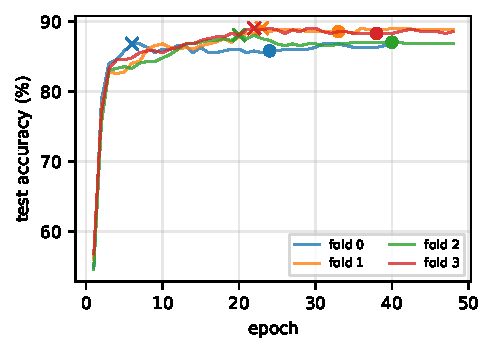
\includegraphics[width=\linewidth]{fig4_selection}
  \caption{Test accuracy after every epoch for the four folds of X3D-M
  with the final recipe, never used for any decision. Circles: the epoch
  chosen on the validation fold; crosses: the best test epoch, which is
  what selecting on the test split would report.}
  \label{fig:selection}
\end{figure}

Every run logs test accuracy after each epoch, without using it for any
decision. Choosing the epoch on the test split instead of on the
validation fold would raise the reported single-model accuracy by 0.38 to
1.38 points depending on the model (mean 0.81, maximum over folds 1.75).
On top of this, nine training clips of the official RWF-2000 release are
copies of test clips, so a model trained on that release has seen part of
its test set. An improvement of one point on this
benchmark is therefore within the range that the evaluation procedure
alone can produce, which is the reason for the protocol of
Section~\ref{sec:protocol}.

\subsection{Transfer between datasets}
\label{sec:cross}

Table~\ref{tab:cross} applies every model to the test splits of the other
two datasets without any adaptation. In-domain accuracy says little about
what happens then: a detector trained on Hockey Fights, where it reaches
96\%, falls to 64--65\% on RWF-2000, and one trained on RLVS, where it
reaches 98\%, falls to 59\% on Hockey Fights. The three benchmarks measure
different things, which is a reason to be careful with results reported on
a single one of them. The teacher transfers better than the compact models
when it is trained on the smallest dataset (74.6 against 63.6 from Hockey
to RWF-2000), and the modules give a small advantage in five of the six
transfer directions (mean $+0.65$ points), the one consistent signal we
observe in their favour besides Hockey Fights.

\begin{table}[t]
  \centering
  \caption{Transfer: test accuracy of single models trained on the row
  dataset and applied to the column dataset without adaptation (final
  recipe, mean over fold models). In-domain results in brackets.}
  \label{tab:cross}
  \setlength{\tabcolsep}{2.5pt}
  \begin{tabular}{llccc}
    \toprule
    Trained on & Model & RWF-2000 & Hockey & RLVS \\
    \midrule
    RWF-2000 & X3D-M      & (87.4) & 74.9 & 88.0 \\
             & MA-X3D     & (87.6) & 76.0 & 88.3 \\
             & VideoMAE-B & (91.2) & 67.2 & 90.7 \\
    Hockey   & X3D-M      & 63.6 & (96.1) & 67.8 \\
             & MA-X3D     & 65.4 & (95.6) & 65.9 \\
             & VideoMAE-B & 74.6 & (94.9) & 76.1 \\
    RLVS     & X3D-M      & 79.7 & 58.5 & (98.5) \\
             & MA-X3D     & 81.2 & 59.6 & (98.2) \\
    \bottomrule
  \end{tabular}
\end{table}

\subsection{Inference options}
\label{sec:options}

On the OOF predictions, four temporal views raise accuracy by 0.25 points
over a single view (0.4 points on the test split) at four times the cost;
horizontal-flip augmentation lowers OOF accuracy slightly; tuning the
threshold on $[0.30, 0.70]$ selects 0.50--0.52 and brings no measurable
gain. Averaging the four fold models, which multiplies the cost by four
again, gives 89.25\% test accuracy. We report the single model with one
view as the deployed configuration.

\subsection{Cost}

The deployed model has 3.01M parameters and 6.46 GFLOPs per view against
86.2M and 135 for the teacher, and needs 208\,ms against 400\,ms per clip
on an AMD EPYC 7413 CPU with 16 threads. On the MI250 GPU the two have
similar latency (30 and 24\,ms at batch 1, 118 and 136 clips/s at batch 16
in fp16):
channel-wise 3D convolutions are limited by memory bandwidth, while the
dense matrix products of the transformer run close to peak. The advantage of the compact model is therefore largest on CPUs and
memory-limited devices, which is where a per-camera detector runs. INT8
quantisation with ONNX Runtime is not useful here: it doubles CPU latency,
because channel-wise 3D convolutions have no efficient integer kernels,
and costs 1.5 points of accuracy. Training one fold takes 48 minutes for
the student and 12 for the teacher on one GCD, at 5.8 and 9.4 GB.


\subsection{Qualitative analysis}

% TODO: Grad-CAM with and without Motion Attention, gate maps, error cases.
The gate reacts to the class: the mean absolute gain $|G|$ over the OOF
clips is 0.059 on violent clips and 0.050 on non-violent ones, so the
modulation of the Res4 features stays within a few per cent and is
slightly stronger when violence is present.

\section{Recommendations}

The measurements above suggest four practices for work on these benchmarks,
none of which costs more than the experiments already being run.
\emph{Audit the split.} Nine training clips of RWF-2000 are copies of test
clips, and the copy of RLVS we obtained stores every video twice; a
descriptor comparison takes minutes and the split files can be released.
\emph{State how the checkpoint is chosen.} On our runs, choosing the epoch
on the test split adds 0.8 points, which is more than most reported
architectural gains. \emph{Report more than one seed.} A single seed
produced a significant $+1.25$ points on Hockey Fights that three seeds
removed. \emph{Compare at a matched cost and a matched recipe.} A tuned
training schedule is worth 2.80 points here, so a module compared against
an under-trained baseline will appear to work even when it does not.

All splits, audit files, configurations, seeds and training code are
released, together with the per-clip out-of-fold predictions used for every
test in this paper, so each number can be recomputed without retraining.

%======================================================================
\section{Limitations}

Our conclusions rest on three datasets of 1{,}000 to 2{,}000 clips, whose
test splits hold 200 to 400 clips, so one point is two to four clips; this
is why we report paired tests. The modules were evaluated in the
configuration proposed for them and on one backbone family, so our finding
that they do not help a tuned X3D-M is not a statement about motion cues in
general. The distillation study uses one teacher, and the control shows
that most of its effect is the longer schedule. Test accuracy is 1--3 points below
out-of-fold accuracy for every model, including the teacher, which
suggests that the test clips are harder than the training clips rather
than that the models overfit the folds. Finally, the person-centred crop
assumes a fixed camera, and all models classify trimmed clips without
localising the event in time.

%======================================================================
\section{Conclusion}
\label{sec:conclusion}

We asked what actually improves a compact violence detector, and measured
each candidate under a protocol that removes duplicated clips, keeps clips
of the same scene in one fold, decides out of fold and scores each test
split once. The answer is not where this literature has been looking. The
input pipeline that the task inherits---detect people, crop to them,
equalise contrast---costs 2.97 out-of-fold points, more than every module
and the training recipe together, and the pipeline that replaces it has no
detector in it at all. Within the network, widening the channel-wise
kernels of every stage is worth 2.63 test points over three seeds at 25\%
more computation and no extra inference machinery, while the same widening
confined to the first two stages, as the original design has it, is worth
0.75. A motion-attention gate is worth nothing, and the control that feeds
it an all-zero motion map settles why: the gate never used its motion
input. Two effects outside the model remain of the same order as the
modules, namely 0.8 points for choosing the epoch on the test split and a
significant single-seed result on Hockey Fights that three seeds erase.

The resulting detector reaches 91.6\% on RWF-2000 over three seeds with
3.3M parameters and 5.9 GFLOPs per view, deployed as the weight average of
the four fold models that the protocol trains anyway, which is as accurate
as their ensemble at a quarter of its cost. We release the splits, the duplicate audit, the seven rebuilt
pipelines and the training code, so that the next lightweight detector can
be compared on the same basis rather than on numbers whose protocol is
unknown.

\bibliographystyle{IEEEtran}
\bibliography{refs}

\end{document}
